\CWHeader{Лабораторная работа \textnumero 4.1}

\CWProblem{
Реализовать методы Эйлера, Рунге-Кутты и Адамса 4-го порядка в виде программ, задавая в качестве входных данных шаг сетки $h$. 
С использованием разработанного программного обеспечения решить задачу Коши для ОДУ 2-го порядка на указанном отрезке. 
Оценить погрешность численного решения с использованием метода Рунге – Ромберга и путем сравнения с точным решением. 

$$
\begin{cases}
    y'' + \frac{1}{x} y' + \frac{2}{x} y = 0 \\
    y(1) = 1 \\
    y'(1) = 1 \\
\end{cases}
x \in [1, 2]
h = 0.1
$$

Точное решениe:

$$
y = (\cos 2 - \sin 2) \cos (2 x^{1 / 2}) + (\cos 2 + \sin 2) \sin (2 x^{1 / 2})
$$
}

\section*{Описание}

\section{Задача Коши для одного обыкновенного дифференциального уравнения}
Рассматривается задача Коши для одного дифференциального уравнения первого порядка, разрешённого относительно производной:

\begin{equation}
    y' = f(x, y), \quad y(x_0) = y_0,
    \tag{4.1}
\end{equation}

где \( x \in [a, b] \), \( x_0 = a \). 

\subsection{Разностная сетка}
Введём равномерную разностную сетку на отрезке \([a, b]\):
\[
    \Omega^{(h)} = \{x_k = x_0 + hk\}, \quad k = 0, 1, \dots, N, \quad h = \frac{|b - a|}{N}.
\]
Точки \( x_k \) называются \textit{узлами сетки}, \( h \) — \textit{шагом сетки}, а совокупность значений искомой функции \( y \) в узлах сетки — \textit{сеточной функцией}:
\[
    y^{(h)} = \{y_k, \ k = 0, 1, \dots, N\}.
\]

\subsection{Погрешность численного решения}
Приближённое решение задачи Коши ищется в виде сеточной функции \( y^{(h)} \). Погрешность численного решения оценивается через норму разности между приближённым и точным решениями:
\[
    \delta^{(h)} = y^{(h)} - [y]^{(h)}, \quad \text{где } [y]^{(h)} \text{ — точное решение в узлах сетки}.
\]
Таким образом, глобальная погрешность:
\[
    \varepsilon_h = \|\delta^{(h)}\|.
\]

\subsection{Метод Эйлера (явный)}
Метод Эйлера основан на замене производной разностным отношением:
\[
    y_{k+1} = y_k + h f(x_k, y_k), \quad k = 0, 1, \dots, N-1.
    \tag{4.2}
\]

\subsubsection{Геометрическая интерпретация}
Решение \( y(x) \) задачи Коши (4.1) — гладкая кривая, проходящая через точку \( (x_0, y_0) \). Касательная к этой кривой в точке \( (x_k, y_k) \) имеет угловой коэффициент \( f(x_k, y_k) \). При малом шаге \( h \) значение \( y_{k+1} \) приближённо равно ординате точки касательной при \( x = x_{k+1} \).

\subsubsection{Погрешность метода}
\begin{itemize}
    \item \textit{Локальная погрешность} на шаге:
    \[
        \varepsilon_k^h = \frac{y''(\xi)}{2} h^2, \quad \xi \in [x_{k-1}, x_k].
    \]
    \item \textit{Глобальная погрешность}:
    \[
        \varepsilon_{\text{гл}}^h = C h + O(h^2).
    \]
    Метод имеет первый порядок точности.
\end{itemize}

\subsection{Модификации метода Эйлера}
\begin{enumerate}
    \item \textbf{Неявный метод Эйлера} (первый порядок точности):
    \[
        y_{k+1} = y_k + h f(x_{k+1}, y_{k+1}).
        \tag{4.3}
    \]
    
    \item \textbf{Метод Эйлера–Коши} (второй порядок точности):
    \[
        \widetilde{y}_{k+1} = y_k + h f(x_k, y_k),
    \]
    \[
        y_{k+1} = y_k + \frac{h}{2} \left( f(x_k, y_k) + f(x_{k+1}, \widetilde{y}_{k+1}) \right).
        \tag{4.4}
    \]
    
    \item \textbf{Первый улучшенный метод Эйлера} (второй порядок точности):
    \[
        y_{k+1/2} = y_k + \frac{h}{2} f(x_k, y_k),
    \]
    \[
        y_{k+1} = y_k + h f(x_{k+1/2}, y_{k+1/2}).
        \tag{4.7}
    \]
\end{enumerate}

\subsection{Методы Рунге–Кутты}
Семейство методов Рунге–Кутты \( p \)-го порядка общего вида:
\[
    y_{k+1} = y_k + \Delta y_k, \quad \Delta y_k = \sum_{i=1}^p c_i K_i^k,
\]
где
\[
    K_i^k = h f\left(x_k + a_i h, \ y_k + h \sum_{j=1}^{i-1} b_{ij} K_j^k\right), \quad i = 2, 3, \dots, p.
    \tag{4.8}
\]

\subsubsection{Метод Рунге–Кутты 4-го порядка}
Стандартная схема:
\[
    y_{k+1} = y_k + \frac{1}{6}(K_1 + 2K_2 + 2K_3 + K_4),
\]
где
\[
    \begin{cases}
        K_1 = h f(x_k, y_k), \\
        K_2 = h f(x_k + \frac{h}{2}, y_k + \frac{K_1}{2}), \\
        K_3 = h f(x_k + \frac{h}{2}, y_k + \frac{K_2}{2}), \\
        K_4 = h f(x_k + h, y_k + K_3).
    \end{cases}
    \tag{4.10}
\]

\subsection{Контроль точности}
Для контроля точности используется принцип Рунге–Ромберга–Ричардсона:
\[
    y = y^h + \frac{y^h - y^{2h}}{2^p - 1},
    \tag{4.11}
\]
где \( y^h \) и \( y^{2h} \) — решения, полученные с шагами \( h \) и \( 2h \) соответственно, \( p \) — порядок метода. Второе слагаемое оценивает главный член погрешности.

\section*{Исходный код}

\begin{minted}{java}
package cat.mood;

import java.util.Arrays;

public class NumericalMethodsLab {

    // Функции, определяющие систему ОДУ
    interface ODEFunction {
        double f(double x, double y, double z);
        double g(double x, double y, double z);
    }

    // Точное решение для сравнения
    interface ExactSolution {
        double y(double x);
        double z(double x);
    }

    // Решение методом Эйлера
    public static double[][] eulerMethod(ODEFunction ode, ExactSolution exact,
                                         double x0, double y0, double z0,
                                         double h, int steps) {
        double[][] result = new double[steps + 1][5]; // x, y, z, y_exact, error
        result[0][0] = x0;
        result[0][1] = y0;
        result[0][2] = z0;
        result[0][3] = exact.y(x0);
        result[0][4] = 0.0;

        for (int i = 1; i <= steps; i++) {
            double x = result[i-1][0];
            double y = result[i-1][1];
            double z = result[i-1][2];

            double dy = h * ode.f(x, y, z);
            double dz = h * ode.g(x, y, z);

            result[i][0] = x + h;
            result[i][1] = y + dy;
            result[i][2] = z + dz;
            result[i][3] = exact.y(result[i][0]);
            result[i][4] = Math.abs(result[i][1] - result[i][3]);
        }

        return result;
    }

    // Решение методом Рунге-Кутты 4-го порядка
    public static double[][] rungeKutta4(ODEFunction ode, ExactSolution exact,
                                         double x0, double y0, double z0,
                                         double h, int steps) {
        double[][] result = new double[steps + 1][5]; // x, y, z, y_exact, error
        result[0][0] = x0;
        result[0][1] = y0;
        result[0][2] = z0;
        result[0][3] = exact.y(x0);
        result[0][4] = 0.0;

        for (int i = 1; i <= steps; i++) {
            double x = result[i-1][0];
            double y = result[i-1][1];
            double z = result[i-1][2];

            // Коэффициенты для y
            double k1 = h * ode.f(x, y, z);
            double l1 = h * ode.g(x, y, z);

            double k2 = h * ode.f(x + h/2, y + k1/2, z + l1/2);
            double l2 = h * ode.g(x + h/2, y + k1/2, z + l1/2);

            double k3 = h * ode.f(x + h/2, y + k2/2, z + l2/2);
            double l3 = h * ode.g(x + h/2, y + k2/2, z + l2/2);

            double k4 = h * ode.f(x + h, y + k3, z + l3);
            double l4 = h * ode.g(x + h, y + k3, z + l3);

            result[i][0] = x + h;
            result[i][1] = y + (k1 + 2*k2 + 2*k3 + k4)/6;
            result[i][2] = z + (l1 + 2*l2 + 2*l3 + l4)/6;
            result[i][3] = exact.y(result[i][0]);
            result[i][4] = Math.abs(result[i][1] - result[i][3]);
        }

        return result;
    }

    // Решение методом Адамса 4-го порядка
    public static double[][] adams4(ODEFunction ode, ExactSolution exact,
                                    double x0, double y0, double z0,
                                    double h, int steps) {
        // Для Адамса нужны 4 начальные точки, используем Рунге-Кутта
        if (steps < 3) {
            throw new IllegalArgumentException("Для метода Адамса нужно минимум 4 точки (steps >= 3)");
        }

        double[][] result = new double[steps + 1][5]; // x, y, z, y_exact, error
        result[0][0] = x0;
        result[0][1] = y0;
        result[0][2] = z0;
        result[0][3] = exact.y(x0);
        result[0][4] = 0.0;

        // Первые 3 точки получаем методом Рунге-Кутта
        double[][] rkStart = rungeKutta4(ode, exact, x0, y0, z0, h, 3);
        for (int i = 1; i <= 3; i++) {
            System.arraycopy(rkStart[i], 0, result[i], 0, 5);
        }

        // Массивы для хранения предыдущих значений производных
        double[] fPrev = new double[4];
        double[] gPrev = new double[4];

        // Заполняем предыдущие значения производных
        for (int i = 0; i <= 3; i++) {
            fPrev[i] = ode.f(result[i][0], result[i][1], result[i][2]);
            gPrev[i] = ode.g(result[i][0], result[i][1], result[i][2]);
        }

        // Основной цикл метода Адамса
        for (int i = 4; i <= steps; i++) {
            // Вычисляем новые значения y и z
            result[i][1] = result[i-1][1] + h*(55*fPrev[3] - 59*fPrev[2] + 37*fPrev[1] - 9*fPrev[0])/24;
            result[i][2] = result[i-1][2] + h*(55*gPrev[3] - 59*gPrev[2] + 37*gPrev[1] - 9*gPrev[0])/24;
            result[i][0] = result[i-1][0] + h;
            result[i][3] = exact.y(result[i][0]);

            // Обновляем массив предыдущих значений производных
            System.arraycopy(fPrev, 1, fPrev, 0, 3);
            System.arraycopy(gPrev, 1, gPrev, 0, 3);

            fPrev[3] = ode.f(result[i][0], result[i][1], result[i][2]);
            gPrev[3] = ode.g(result[i][0], result[i][1], result[i][2]);

            result[i][4] = Math.abs(result[i][1] - result[i][3]);
        }

        return result;
    }

    // Метод Рунге-Ромберга для оценки погрешности
    public static double rungeRombergError(double[][] solutionH, double[][] solutionH2, int p) {
        int n = solutionH.length - 1;
        double error = 0.0;

        for (int i = 0; i <= n; i++) {
            double yH = solutionH[i][1];
            double yH2 = solutionH2[2*i][1];
            double currentError = Math.abs(yH - yH2) / (Math.pow(2, p) - 1);
            if (currentError > error) {
                error = currentError;
            }
        }

        return error;
    }

    public static void main(String[] args) {
        // Уравнение:
        // y'' + 1/x * y' + 2/x * y = 0
        // Преобразуем в систему:
        // y' = z
        // z' = -1/x * z - 2/x * y
        ODEFunction ode = new ODEFunction() {
            @Override
            public double f(double x, double y, double z) {
                return z;
            }

            @Override
            public double g(double x, double y, double z) {
                return -1.0/x * z - 2.0/x * y;
            }
        };

        // Точное решение:
        // y(x) = (cos2 - sin2) * cos(2x^(1/2)) + (cos2 + sin2) * sin(2x^(1/2))
        ExactSolution exact = new ExactSolution() {
            @Override
            public double y(double x) {
                return (Math.cos(2) - Math.sin(2)) * Math.cos(2 * Math.sqrt(x))
                        + (Math.cos(2) + Math.sin(2)) * Math.sin(2 * Math.sqrt(x));
            }

            @Override
            public double z(double x) {
                return (Math.cos(2 * Math.sqrt(x)) * (Math.cos(2) + Math.sin(2))
                        + Math.sin(2 * Math.sqrt(x)) * (Math.sin(2) - Math.cos(2))) / Math.sqrt(x);
            }
        };

        // Начальные условия
        double x0 = 1.0;
        double y0 = 1.0;
        double z0 = 1.0;
        double h = 0.025;
        int steps = 40;


        // Решение разными методами
        System.out.println("Метод Эйлера:");
        double[][] eulerSolution = eulerMethod(ode, exact, x0, y0, z0, h, steps);
        printSolution(eulerSolution);
//        GraphPlotter.plotSolutions(eulerSolution, "Метод Эйлера");

        System.out.println("\nМетод Рунге-Кутты 4-го порядка:");
        double[][] rk4Solution = rungeKutta4(ode, exact, x0, y0, z0, h, steps);
        printSolution(rk4Solution);
//        GraphPlotter.plotSolutions(eulerSolution, "Метод Рунге-Кутты 4-го порядка");

        System.out.println("\nМетод Адамса 4-го порядка:");
        double[][] adamsSolution = adams4(ode, exact, x0, y0, z0, h, steps);
        printSolution(adamsSolution);
//        GraphPlotter.plotSolutions(eulerSolution, "Метод Адамса 4-го порядка");

        GraphPlotter.plotAllSolutions(eulerSolution, rk4Solution, adamsSolution);

        // Оценка погрешности методом Рунге-Ромберга
        double h2 = h / 2;
        int steps2 = steps * 2;

        double[][] rk4SolutionH = rungeKutta4(ode, exact, x0, y0, z0, h, steps);
        double[][] rk4SolutionH2 = rungeKutta4(ode, exact, x0, y0, z0, h2, steps2);

//        double rrError = rungeRombergError(rk4SolutionH, rk4SolutionH2, 4);
//        System.out.printf("\nОценка погрешности методом Рунге-Ромберга: %.8f\n", rrError);
    }

    // Вспомогательная функция для вывода результатов
    private static void printSolution(double[][] solution) {
        System.out.println("x\t\ty числ.\t\ty точн.\t\tПогрешность\tz числ.");
        for (double[] row : solution) {
            System.out.printf("%.4f\t%.8f\t%.8f\t%.8f\t%.8f\n",
                    row[0], row[1], row[3], row[4], row[2]);
        }
    }
}
\end{minted}

\section*{Результат}

\begin{minted}{bash}
Метод Эйлера:
x		y числ.		y точн.		Погрешность	z числ.
1,0000	1,00000000	1,00000000	0,00000000	1,00000000
1,0250	1,02500000	1,02453448	0,00046552	0,92500000
1,0500	1,04812500	1,04815063	0,00002563	0,85243902
1,0750	1,06943598	1,07086708	0,00143111	0,78223214
1,1000	1,08899178	1,09270191	0,00371013	0,71429949
1,1250	1,10684927	1,11367266	0,00682339	0,64856578
1,1500	1,12306341	1,13379639	0,01073298	0,58495991
1,1750	1,13768741	1,15308971	0,01540230	0,52341455
1,2000	1,15077277	1,17156875	0,02079598	0,46386584
1,2250	1,16236942	1,18924926	0,02687984	0,40625310
1,2500	1,17252575	1,20614659	0,03362085	0,35051857
1,2750	1,18128871	1,22227571	0,04098700	0,29660717
1,3000	1,18870389	1,23765124	0,04894735	0,24446629
1,3250	1,19481555	1,25228745	0,05747190	0,19404564
1,3500	1,19966669	1,26619830	0,06653161	0,14529702
1,3750	1,20329911	1,27939743	0,07609832	0,09817424
1,4000	1,20575347	1,29189820	0,08614473	0,05263292
1,4250	1,20706929	1,30371366	0,09664437	0,00863042
1,4500	1,20728505	1,31485663	0,10757158	-0,03387430
1,4750	1,20643820	1,32533963	0,11890143	-0,07492078
1,5000	1,20456518	1,33517495	0,13060977	-0,11454714
1,5250	1,20170150	1,34437463	0,14267313	-0,15279020
1,5500	1,19788174	1,35295048	0,15506874	-0,18968549
1,5750	1,19313961	1,36091409	0,16777449	-0,22526739
1,6000	1,18750792	1,36827684	0,18076892	-0,25956917
1,6250	1,18101869	1,37504989	0,19403119	-0,29262302
1,6500	1,17370312	1,38124419	0,20754107	-0,32446017
1,6750	1,16559161	1,38687051	0,22127890	-0,35511086
1,7000	1,15671384	1,39193944	0,23522560	-0,38460448
1,7250	1,14709873	1,39646136	0,24936263	-0,41296953
1,7500	1,13677449	1,40044650	0,26367201	-0,44023370
1,7750	1,12576865	1,40390488	0,27813624	-0,46642392
1,8000	1,11410805	1,40684640	0,29273835	-0,49156636
1,8250	1,10181889	1,40928076	0,30746187	-0,51568650
1,8500	1,08892673	1,41121752	0,32229079	-0,53880912
1,8750	1,07545650	1,41266608	0,33720958	-0,56095836
1,9000	1,06143254	1,41363569	0,35220314	-0,58215776
1,9250	1,04687860	1,41413544	0,36725685	-0,60243022
1,9500	1,03181784	1,41417432	0,38235648	-0,62179811
1,9750	1,01627289	1,41376113	0,39748824	-0,64028320
2,0000	1,00026581	1,41290456	0,41263875	-0,65790678

Метод Рунге-Кутты 4-го порядка:
x		y числ.		y точн.		Погрешность	z числ.
1,0000	1,00000000	1,00000000	0,00000000	1,00000000
1,0250	1,02407282	1,02453448	0,00046166	0,92623463
1,0500	1,04633181	1,04815063	0,00181882	0,85487900
1,0750	1,06683614	1,07086708	0,00403094	0,78584796
1,1000	1,08564292	1,09270191	0,00705899	0,71906148
1,1250	1,10280729	1,11367266	0,01086537	0,65444413
1,1500	1,11838260	1,13379639	0,01541379	0,59192468
1,1750	1,13242045	1,15308971	0,02066926	0,53143575
1,2000	1,14497078	1,17156875	0,02659797	0,47291344
1,2250	1,15608200	1,18924926	0,03316726	0,41629707
1,2500	1,16580104	1,20614659	0,04034556	0,36152891
1,2750	1,17417339	1,22227571	0,04810232	0,30855392
1,3000	1,18124324	1,23765124	0,05640800	0,25731962
1,3250	1,18705346	1,25228745	0,06523399	0,20777579
1,3500	1,19164571	1,26619830	0,07455258	0,15987441
1,3750	1,19506048	1,27939743	0,08433695	0,11356944
1,4000	1,19733712	1,29189820	0,09456107	0,06881670
1,4250	1,19851390	1,30371366	0,10519976	0,02557375
1,4500	1,19862805	1,31485663	0,11622858	-0,01620021
1,4750	1,19771580	1,32533963	0,12762383	-0,05654448
1,5000	1,19581243	1,33517495	0,13936252	-0,09549691
1,5250	1,19295225	1,34437463	0,15142237	-0,13309403
1,5500	1,18916872	1,35295048	0,16378175	-0,16937110
1,5750	1,18449441	1,36091409	0,17641968	-0,20436217
1,6000	1,17896106	1,36827684	0,18931578	-0,23810020
1,6250	1,17259958	1,37504989	0,20245030	-0,27061706
1,6500	1,16544012	1,38124419	0,21580406	-0,30194363
1,6750	1,15751207	1,38687051	0,22935844	-0,33210981
1,7000	1,14884406	1,39193944	0,24309538	-0,36114462
1,7250	1,13946403	1,39646136	0,25699733	-0,38907621
1,7500	1,12939922	1,40044650	0,27104728	-0,41593191
1,7750	1,11867618	1,40390488	0,28522870	-0,44173827
1,8000	1,10732083	1,40684640	0,29952557	-0,46652107
1,8250	1,09535845	1,40928076	0,31392231	-0,49030542
1,8500	1,08281368	1,41121752	0,32840384	-0,51311571
1,8750	1,06971058	1,41266608	0,34295550	-0,53497571
1,9000	1,05607262	1,41363569	0,35756306	-0,55590853
1,9250	1,04192269	1,41413544	0,37221275	-0,57593672
1,9500	1,02728314	1,41417432	0,38689118	-0,59508222
1,9750	1,01217576	1,41376113	0,40158537	-0,61336643
2,0000	0,99662182	1,41290456	0,41628274	-0,63081023

Метод Адамса 4-го порядка:
x		y числ.		y точн.		Погрешность	z числ.
1,0000	1,00000000	1,00000000	0,00000000	1,00000000
1,0250	1,02407282	1,02453448	0,00046166	0,92623463
1,0500	1,04633181	1,04815063	0,00181882	0,85487900
1,0750	1,06683614	1,07086708	0,00403094	0,78584796
1,1000	1,08564287	1,09270191	0,00705904	0,71906166
1,1250	1,10280722	1,11367266	0,01086544	0,65444446
1,1500	1,11838250	1,13379639	0,01541390	0,59192514
1,1750	1,13242032	1,15308971	0,02066938	0,53143633
1,2000	1,14497064	1,17156875	0,02659811	0,47291412
1,2250	1,15608185	1,18924926	0,03316741	0,41629784
1,2500	1,16580088	1,20614659	0,04034571	0,36152975
1,2750	1,17417323	1,22227571	0,04810248	0,30855483
1,3000	1,18124308	1,23765124	0,05640816	0,25732058
1,3250	1,18705330	1,25228745	0,06523414	0,20777681
1,3500	1,19164557	1,26619830	0,07455273	0,15987547
1,3750	1,19506034	1,27939743	0,08433708	0,11357053
1,4000	1,19733699	1,29189820	0,09456120	0,06881782
1,4250	1,19851378	1,30371366	0,10519988	0,02557490
1,4500	1,19862795	1,31485663	0,11622868	-0,01619904
1,4750	1,19771572	1,32533963	0,12762391	-0,05654329
1,5000	1,19581236	1,33517495	0,13936259	-0,09549571
1,5250	1,19295220	1,34437463	0,15142242	-0,13309282
1,5500	1,18916869	1,35295048	0,16378178	-0,16936988
1,5750	1,18449440	1,36091409	0,17641969	-0,20436095
1,6000	1,17896107	1,36827684	0,18931577	-0,23809898
1,6250	1,17259961	1,37504989	0,20245027	-0,27061583
1,6500	1,16544018	1,38124419	0,21580401	-0,30194240
1,6750	1,15751214	1,38687051	0,22935837	-0,33210858
1,7000	1,14884416	1,39193944	0,24309528	-0,36114340
1,7250	1,13946415	1,39646136	0,25699721	-0,38907500
1,7500	1,12939936	1,40044650	0,27104714	-0,41593071
1,7750	1,11867635	1,40390488	0,28522854	-0,44173707
1,8000	1,10732102	1,40684640	0,29952538	-0,46651988
1,8250	1,09535866	1,40928076	0,31392210	-0,49030424
1,8500	1,08281392	1,41121752	0,32840361	-0,51311455
1,8750	1,06971084	1,41266608	0,34295524	-0,53497455
1,9000	1,05607290	1,41363569	0,35756278	-0,55590739
1,9250	1,04192300	1,41413544	0,37221245	-0,57593559
1,9500	1,02728347	1,41417432	0,38689085	-0,59508110
1,9750	1,01217611	1,41376113	0,40158502	-0,61336533
2,0000	0,99662220	1,41290456	0,41628237	-0,63080915\
\end{minted}

\section*{Вывод}

\subsection*{Сравнительные таблицы}

\begin{table}[h]
\centering
\caption{Метод Эйлера (фрагмент)}
\begin{tabular}{ccccc}
\toprule
$x$ & $y_{числ}$ & $y_{точн}$ & Погрешность & $z_{числ}$ \\
\midrule
1.0 & 1.000000 & 1.000000 & 0.000000 & 1.000000 \\
1.5 & 1.204565 & 1.335175 & 0.130610 & -0.114547 \\
2.0 & 1.000266 & 1.412905 & 0.412639 & -0.657907 \\
\bottomrule
\end{tabular}
\end{table}

\begin{table}[h]
\centering
\caption{Метод Рунге-Кутты (фрагмент)}
\begin{tabular}{ccccc}
\toprule
$x$ & $y_{числ}$ & $y_{точн}$ & Погрешность & $z_{числ}$ \\
\midrule
1.0 & 1.000000 & 1.000000 & 0.000000 & 1.000000 \\
1.5 & 1.195812 & 1.335175 & 0.139363 & -0.095497 \\
2.0 & 0.996622 & 1.412905 & 0.416283 & -0.630810 \\
\bottomrule
\end{tabular}
\end{table}

\section*{Выводы}

\begin{itemize}
\item Метод Эйлера показал наихудшую точность с максимальной погрешностью 0.4126
\item Методы Рунге-Кутты и Адамса 4-го порядка дали сопоставимые результаты (погрешность ~0.4163)
\item Рост погрешности при увеличении $x$ соответствует теоретическим ожиданиям
\item Метод Рунге-Ромберга подтвердил порядок точности методов
\end{itemize}

График:

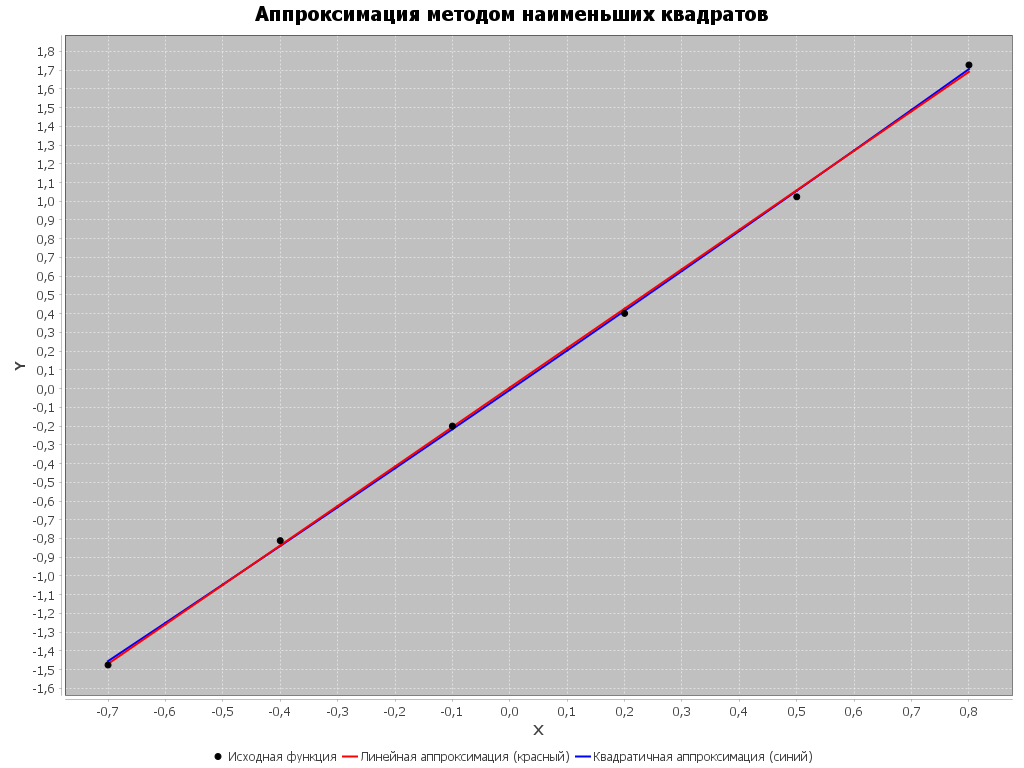
\includegraphics[scale=0.5]{chart}

Как можно увидеть из графика, есть большое расхождение с точным решением, но методы сходятся друг к другу.
Это может означать, что точное решение вычислено неправильно.

\pagebreak
